\documentclass{standalone}

\usepackage{tikz,pgfplots}

\pgfplotsset{compat=1.18}
\pgfplotsset{
	soldot/.style={
		color=black,only marks,mark=*},
	holdot/.style={
		color=black,fill=white,only marks,mark=*},
	compat=1.12,
	standard/.style={
     		every axis x label/.style={at={(current axis.right of origin)},anchor=north west},
    		every axis y label/.style={at={(current axis.above origin)},anchor=north east}}
}

\usetikzlibrary{calc}
\usetikzlibrary{intersections}
\usetikzlibrary{decorations.markings}
\usetikzlibrary{arrows.meta}
\tikzset{>={Latex[scale=1.2]}}

\begin{document}

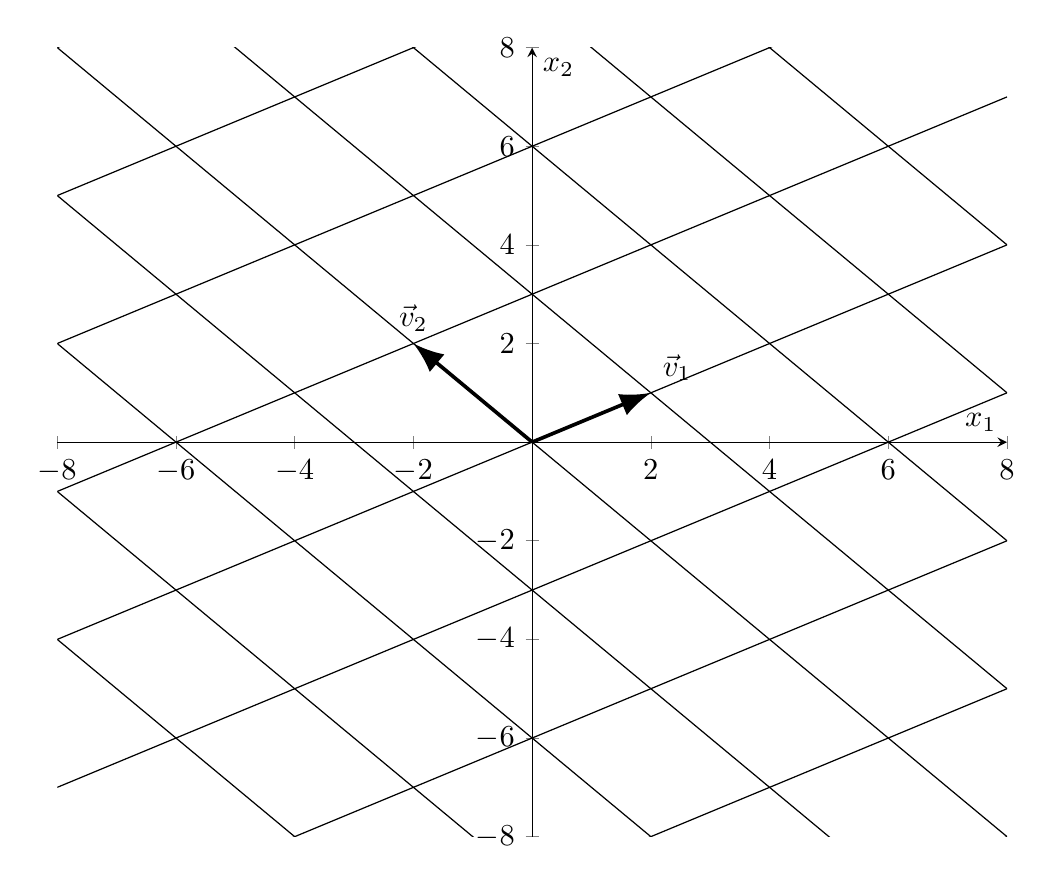
\begin{tikzpicture}[scale=1.1]
\begin{axis}[grid=none,
axis lines=middle,
xmin=-8,xmax=8,
ymin=-8,ymax=8,
xtick={-8,-6,...,8},
ytick={-8,-6,...,8},
minor tick={},
xlabel=\(x_1\), ylabel=\(x_2\),
x post scale = 1.6,
y post scale = 1.6,
samples=250]
\addplot[domain=-8:8] {0.5*x-12};
\addplot[domain=-8:8] {0.5*x-9};
\addplot[domain=-8:8] {0.5*x-6};
\addplot[domain=-8:8] {0.5*x-3};
\addplot[domain=-8:8] {0.5*x};
\addplot[domain=-8:8] {0.5*x+3};
\addplot[domain=-8:8] {0.5*x+6};
\addplot[domain=-8:8] {0.5*x+9};
\addplot[domain=-8:8] {0.5*x+12};

\addplot[domain=-8:8] {-x-12};
\addplot[domain=-8:8] {-x-9};
\addplot[domain=-8:8] {-x-6};
\addplot[domain=-8:8] {-x-3};
\addplot[domain=-8:8] {-x};
\addplot[domain=-8:8] {-x+3};
\addplot[domain=-8:8] {-x+6};
\addplot[domain=-8:8] {-x+9};
\addplot[domain=-8:8] {-x+12};


\draw[->,very thick] (0,0) -- (2,1) node[above right] {$\vec{v}_1$};
\draw[->,very thick] (0,0) -- (-2,2) node[above] {$\vec{v}_2$};

\end{axis}
\end{tikzpicture}

\end{document}